\documentclass{article}
\pdfpagewidth=8.5in
\pdfpageheight=11in

\usepackage{ijcai26}

\usepackage{times}
\usepackage{soul}
\usepackage{url}
\usepackage[hidelinks]{hyperref}
\usepackage[utf8]{inputenc}
\usepackage[small]{caption}
\usepackage{subcaption}
\usepackage{graphicx}
\usepackage{amsmath}
\usepackage{amsthm}
\usepackage{booktabs}
\usepackage{algorithm}
\usepackage{algorithmic}
\usepackage[switch]{lineno}

\linenumbers

\urlstyle{same}

\newtheorem{example}{Example}
\newtheorem{theorem}{Theorem}

\pdfinfo{
/TemplateVersion (IJCAI.2026.0)
}

\title{Radar-based Sentiment Analysis and Recognition}

\author{
Mohamed-anas Abbouchi$^1$
\and
Haider Azam$^2$
\and
Mudassar$^3$
\affiliations
$^1$Aalto University\\
$^2$Second Affiliation\\
$^3$Third Affiliation\\
% \emails
% mohamed-anas.abbouchi@aalto.fi,
% m.haiderazam555@gmail.com,
% third@example.com
}

\begin{document}

\maketitle

\begin{abstract}

\end{abstract}

\section{Introduction}

Sentiment analysis commonly refers to the process of identifying and extracting subjective information from text, speech, or other forms of data \cite{ain2017sentiment}. In this study, we focused on sentiment analysis using radar-based data. Radar sensors are a powerful tool for capturing subtle movements and gestures. They are non-intrusive, privacy-preserving, and much easier to deploy in real-world scenarios compared to other modalities such as cameras or wearable sensors \cite{radargesture2020}. The data from these sensors have proven useful in applications such as gesture recognition \cite{radargesture2020}, object detection \cite{radarobject2018} and human activity recognition \cite{radaractivity2019}. 

The main focus of researchers in the field of sentiment analysis has been on text-based and speech-based data, with a significant amount of work done on NLP models \cite{sentiment2025} and speech processing techniques. The objective was always to create models that understand human emotions through media but rarely through their body movements. Consequently, the use of radar-based data for sentiment analysis and recognition is still a relatively unexplored area, with limited research and few datasets available. The characteristics of radar signals, such as their ability to capture micro-movements and gestures, make them a promising source of information for micro-movement based experiments such as sentiment analysis \cite{radargesture2020}.

The objective of this paper is to explore the potential of radar-based data for sentiment analysis and recognition. We propose different approaches to transform radar signals into training data and evaluate how effective the classification models are in recognizing different sentiments. We split the paper into three experiments, each focusing on a different aspect of the problem. The first experiment focuses on feature-based classification using a mix of kinematic, behavioral and spatial features extracted from the radar signals. The second experiment is based on transformers [FILL HERE]. The third is [FILL HERE].

\section{Related Work}

This research is based on the experiments conducted by \cite{rfbehavior2025}, in which they introduced "a multimodal radio frequency dataset" for both human behavior recognition and emotion analysis. By conducting a series of experiments on 44 participants, they collected data from 13 radars, 8 RFID tags, LoRa devices and infrared cameras in 4 different campaigns that each focused on a different aspect of human behavior. We will be interested in this paper on the third campaign that was built around 6 sentiment states: \textit{depression, distraction, excitement, focus, relaxation and stress}.

\section{Experiment 1: Feature-Based Classification}

\subsection{Preprocessing}

The data is currently composed of a sequence of XYZ coordinates representing the position of a target in 3D space over time. The first step in preprocessing is to synchronize the data from different radar sensors to ensure that the data from different sensors is aligned in time, as this will allow for accurate feature extraction. Once the data is synchronized, the data is normalized on a user basis so the user-specific biases are removed. 

With the data synchronized and normalized, we can proceed to segment the data into smaller windows. This is done to capture the temporal dynamics of the target's movement. The window size and stride are hyperparameters that can be tuned based on the specific application and dataset. In this study, we experimented with different window sizes and strides to find the optimal configuration for our classification task. Lower window sizes tend to underperform and higher window sizes tend to overfit the data and lose generalization. The optimal window size was found to be 90 frames with a stride of 20 frames. This configuration allows for capturing the temporal dynamics of the target's movement while also providing enough data for training the classification models.

\subsection{Feature Extraction}

Given the preprocessed data, we can extract a set of features that capture the kinematic, behavioral and spatial characteristics of the target's movement. The features are extracted from each window of data and are used as input to the classification models. The features are divided into three categories: motion dynamics, statistical and directional features. The motion dynamics features capture the speed, acceleration and jerk of the target's movement. The statistical features capture the distribution of the target's movement in terms of speed, acceleration and jerk. The directional features capture the directionality of the target's movement in terms of turn angles and explained variance ratios. The extracted features are summarized in Tables \ref{tab:dynamics}, \ref{tab:directional} and \ref{tab:behavior}.


\begin{table}[!t]
\centering
\small
\begin{tabular}{p{3.1cm} p{4.2cm}}
\toprule
\textbf{Feature} & \textbf{Description} \\
\midrule
Path Efficiency & Ratio of displacement to trajectory length \\
Mean Speed & Average speed. \\
Std. Speed &  Variability in speed. \\
Median Speed & Median speed. \\
25th Percentile Speed & Lower quartile of speed. \\
75th Percentile Speed & Upper quartile of speed. \\
Mean Acceleration & Average rate of change in speed. \\
Std. Acceleration & Variability of acceleration. \\
Median Acceleration & Median acceleration. \\
25th Percentile Acceleration & Lower quartile of acceleration values. \\
75th Percentile Acceleration & Upper quartile of acceleration values. \\
\bottomrule
\end{tabular}
\caption{Motion dynamics features.}
\label{tab:dynamics}
\end{table}

\begin{table}[!t]
\centering
\small
\begin{tabular}{p{3.1cm} p{4.2cm}}
\toprule
\textbf{Feature} & \textbf{Description} \\
\midrule
Mean Jerk & Average change of acceleration \\
Std. Jerk & Variability in jerk values. \\
Median Jerk & Median jerk. \\
25th Percentile Jerk & Lower quartile of jerk values. \\
75th Percentile Jerk & Upper quartile of jerk values. \\
Spectral Centroid & Center of mass of the movement frequency spectrum. \\
Spectral Entropy & Complexity of the frequency spectrum. \\
Speed CV & Normalized measure of speed variability. \\
Direction Change Rate & Rate of changes in movement direction. \\
Speed Autocorrelation &  Temporal dependence of cursor speed. \\
Tortuosity & Degree of path curvature relative to its overall length. \\
\bottomrule
\end{tabular}
\caption{Statistical and directional features.}
\label{tab:directional}
\end{table}

\begin{table}[!t]
\centering
\small
\begin{tabular}{p{3.1cm} p{4.2cm}}
\toprule
\textbf{Feature} & \textbf{Description} \\
\midrule
Speed Skewness & Asymmetry of the speed distribution. \\
Fraction Stationary Time & Proportion the target remains stationary. \\
Mean Turn Angle & Average angle between consecutive movement segments. \\
Turn Angle Entropy & Diversity and unpredictability of turning angles. \\
Explained Variance Ratio 1 & Variance explained by the first principal component of the trajectory. \\
Explained Variance Ratio 2 & Variance explained by the second principal component. \\
Explained Variance Ratio 3 & Variance explained by the third principal component. \\
\bottomrule
\end{tabular}
\caption{Statistical and directional features.}
\label{tab:behavior}
\end{table}

\subsection{Training Loop}

With the current setup, the data is now composed of 27 features per radar sensor. Given that we have 13 radar sensors, the total number of features is 351 over more than 600 windows. For an effective training of the classification models, we need to reduce the dimensionality of the data and select the most relevant features. To find the optimal configuration of window size, stride and number of features, we implemented a training loop that iterates over different configurations and evaluates the performance of the classification models using Leave-One-Subject-Out (LOSO) cross-validation. It uses the ANOVA F-test to select the top-$k$ features for each radar sensor and concatenates them to form the final feature set. The classification models are then trained on the training set and evaluated on the test set. The accuracy and weighted F1-score are recorded for each configuration and the best configuration is selected based on the highest mean accuracy across all folds. The training loop is summarized in Algorithm \ref{alg:feature_selection}.

\begin{algorithm}[!t]
\caption{Feature Selection and LOSO Classification}
\label{alg:feature_selection}
\begin{algorithmic}
\FOR{each window configuration $(w,s)$}
    \FOR{each feature count $k \in K$}
        \FOR{each Leave-One-Subject-Out split}
            \STATE Split the data into training and testing sets.
            \FOR{each radar $r = 1,\ldots,13$}
                \STATE Select the top-$k$ features using the ANOVA F-test.
                \STATE Transform the training and testing feature sets.
            \ENDFOR
            \STATE Concatenate the selected features from all radars.
            \FOR{each classifier $m \in \mathcal{M}$}
                \STATE Train classifier $m$.
                \STATE Evaluate on the test set.
                \STATE Record the accuracy and weighted F1-score.
            \ENDFOR
        \ENDFOR
        \STATE Compute the mean accuracy and weighted F1-score across all folds.
    \ENDFOR
\ENDFOR
\FOR{each classifier}
    \STATE Select the configuration with the highest mean accuracy.
\ENDFOR
\STATE \textbf{Output:} Best window size, stride, feature count, accuracy, and weighted F1-score for each classifier.
\end{algorithmic}
\end{algorithm}

\subsection{Results}

The best configuration for each model is selected based on the highest mean f1-score across all folds. As previously mentioned, the most optimal configuration across all models was found to be a window size of 90 frames, a stride of 20. The results of the training loop in Figure \ref{fig:models_comparison} are based on models trained with this configuration. 

It shows that the SVM model outperforms the other models with a mean f1-score of 0.72, followed by LightGBM, xGBoost and MLP achieving mean f1-scores in the range of 0.66 and 0.67. The CatBoost classifier underperforms with a mean f1-score of 0.62.

\begin{figure}[!t]
    \centering
    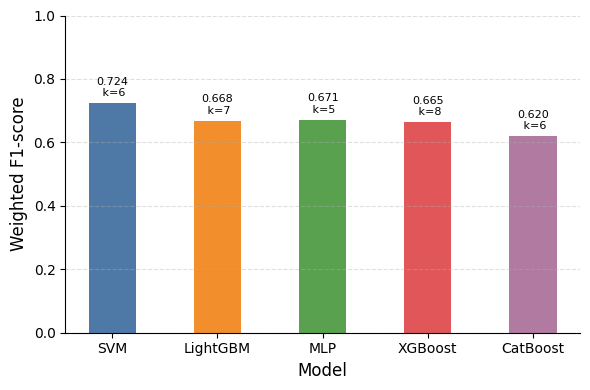
\includegraphics[width=\columnwidth]{figures/models_comparison.png}
    \caption{Models comparison based on F1 score.}
    \label{fig:models_comparison}
\end{figure}

\section{Experiment 2}

\section{Experiment 3: Neural Network-Based Interpolation and Classification}
The radar-based dataset consists of 13 separate radar sensors each recording data at different timestamps, in order to unify the sensors to a single timeline, interpolation is required. This method consists of performing interpolation using Neural Networks and comparing with classical methods, emotion classification is also performed.
\subsection{Preprocessing}
Using the preprocessing sample code provided in the dataset, the radar sensors' data were converted to 39 XYZ coordinates, afterwards, the timestamps were rounded to 1 decimal place and the sensors concatenated together into a single csv file for each user for each emotion. These csv files were then concatenated together to get a singular csv file containing the processed data of every user, emotion and sensor. Grouping by user\_id and emotion, a sparse sequence of observations from all the sensors combined can be retrieved.

To avoid any overlap between dataset splits and to test on unseen users, the user\_ids were split into train, valid and test sets with ratios 0.6/0.2/0.2 . Normalization is performed by setting mean to 0  to allow the model to only train on the residual. Min-max normalization is applied to the timestamps to set the minimum to 0 and maximum to 1.

While training the models, 0.1 to 0.3 of the sequence is randomly set aside as the target, this is set to 0.2 for validation and testing with a static random state for reproducibility. An observation mask containing the non-Nan values is obtained for both the input and target sequence, this is combined with the input sequence to allow the model to focus on observations and is used to train the model using only non-Nan target values. Last Observation Carried Forward (LOCF) is then applied on the data to counter-act the sparsity of the dataset.

\subsection{Model Selection}
The proposed method consists of training a Neural Controlled Differential Equation (NCDE) model by Kidger et. al \cite{kidger2020neuralcde} for interpolation and classification using the torchcde library. It was selected due to it's ability to deal with irregular timestamps. As shown in Figure. \ref{fig:ncde}, the main advantage over Recurrent Neural Networks (RNNs) is the continuous update of it's hidden state, this is achieved by solving and integrating the differential equation in Equation. \ref{eq:differential} where \(f(t,z(t))\) and \(g(x_0)\) are Neual Networks (NNs) and X is a Hermite cubic splines interpolation of sparse input sequence.

\begin{equation}
    \frac{dz(t)}{dt}
    =
    f(t, z(t))
    \frac{dX(t)}{dt},
    \qquad
    z(t_0)=g(x_0),
\label{eq:differential}
\end{equation}

\begin{figure}[!t]
    \centering
    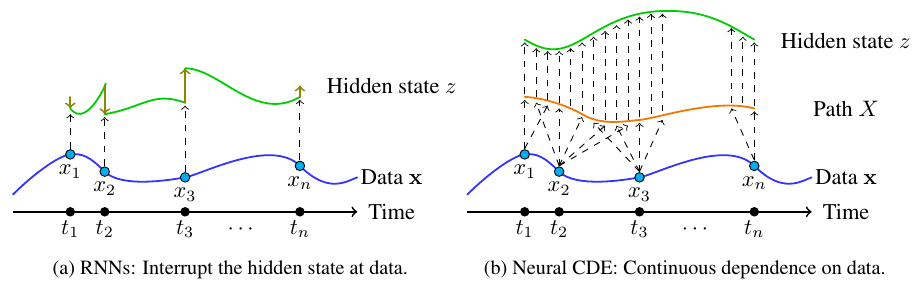
\includegraphics[width=\columnwidth]{figures/NCDE.png}
    \caption{Comparison of hidden state updates between RNN and NCDE.}
    \label{fig:ncde}
\end{figure}

Shown in Figure. \ref{fig:workflow} is the workflow of the proposed method, it starts with interpolating the input sequence using a differentiable hermite cubic spline which is used to obtain a continuous control data X used to obtain z(0) and both are fed into the cdeint function along with the target timestamps dictating at what time we want the hidden states z(t), the entire sequence is fed into an MLP decoder to get the predicted values while the final hidden state is fed into an MLP classifier to get emotion probabilities. Figure. \ref{fig:architecture} shows the various NNs used, Figure. \ref{fig:cdefunc} is the function \(f(t,z(t))\) which is integrated at the target timestamps to get the hidden state at that timestamp, Figure. \ref{fig:encoder} is the function \(g(x)\) used to obtain the initial hidden state z(0), Figure. \ref{fig:decoder} shows the hidden state decoder used to obtain the predicted values at the target timestamps and Figure. \ref{fig:classifier} shows the emotion classifier head.

\begin{figure}[!t]
    \centering
    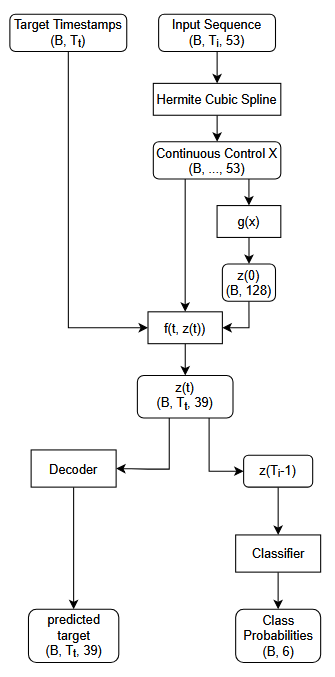
\includegraphics[width=\columnwidth]{figures/workflow.png}
    \caption{Workflow of the proposed method, it uses a differentiable hermite cubic spline which can be integrated to obtain the hidden state at arbitrary timestamps, the final hidden state is used to obtain class probabilities similar to RNNs.}
    \label{fig:workflow}
\end{figure}

\begin{figure}[htbp]
    \centering

    \begin{subfigure}{0.22\textwidth}
        \centering
        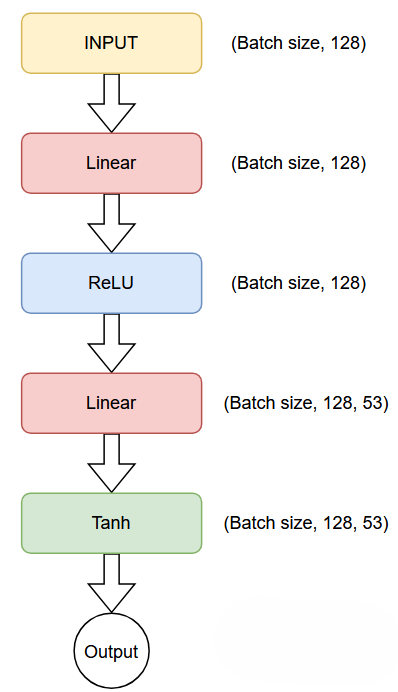
\includegraphics[width=\linewidth]{figures/cde func.png}
        \caption{CDE function f(t, z(t))}
        \label{fig:cdefunc}
    \end{subfigure}
    \hfill
    \begin{subfigure}{0.20\textwidth}
        \centering
        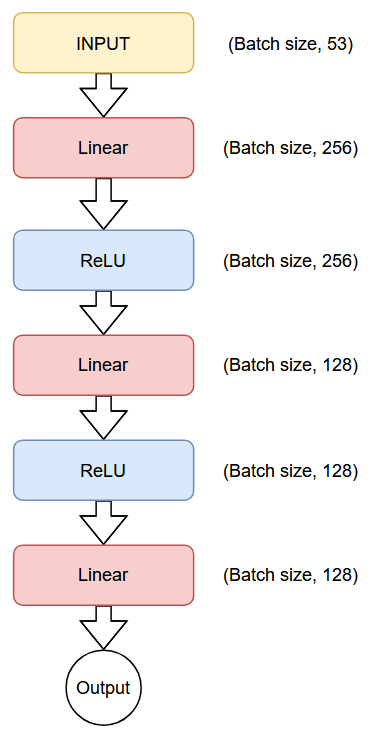
\includegraphics[width=\linewidth]{figures/initial.png}
        \caption{encoder g(x)}
        \label{fig:encoder}
    \end{subfigure}
    
        \vspace{0.5cm}

    \begin{subfigure}{0.20\textwidth}
        \centering
        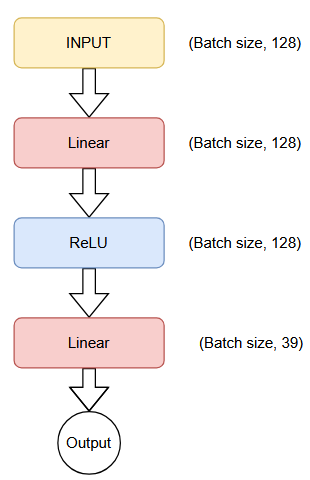
\includegraphics[width=\linewidth]{figures/readout.png}
        \caption{Decoder}
        \label{fig:decoder}
    \end{subfigure}
    \hfill
    \begin{subfigure}{0.20\textwidth}
        \centering
        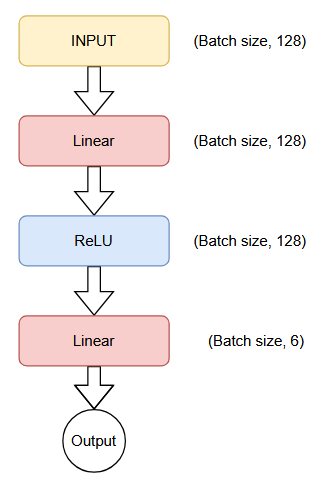
\includegraphics[width=\linewidth]{figures/classifier.png}
        \caption{Emotion Classifier}
        \label{fig:classifier}
    \end{subfigure}

    \caption{The four MLPs used in the model.}
    \label{fig:architecture}
\end{figure}

\subsection{Metrics}
The model was trained using a combination of Mean Squared Error (MSE) loss for the sensor interpolation and, accuracy and cross-entropy loss for the emotion classification.

MSE is shown in Equation. \ref{eq:mse} where \(N\) is the number of reconstructed sensor values, \(y_i\) is the ground truth value, and \(\hat{y}_i\) is the corresponding prediction. Minimizing the MSE encourages the reconstructed values to closely match the original observations.

\begin{equation}
\mathcal{L}_{\text{MSE}}
=
\frac{1}{N}
\sum_{i=1}^{N}
\left(\hat{y}_i-y_i\right)^2,
\label{eq:mse}
\end{equation}

\begin{equation}
\mathcal{L}_{\text{CE}}
=
-
\frac{1}{N}
\sum_{i=1}^{N}
\sum_{c=1}^{C}
y_{i,c}
\log(\hat{p}_{i,c}),
\label{eq:cross-entropy}
\end{equation}

Equation. \ref{eq:cross-entropy} shows the cross-entropy loss where \(C\) is the number of classes, \(y_{i,c}\) is the one-hot encoded ground-truth label for sample \(i\), and \(\hat{p}_{i,c}\) is the predicted probability of class \(c\). The loss penalizes incorrect predictions while encouraging the model to assign high probability to the correct class. In inference, argmax is used to select the class.

\begin{equation}
\text{Accuracy}
=
\frac{\text{Number of Correct Predictions}}
{\text{Total Number of Predictions}}
=
\frac{1}{N}
\sum_{i=1}^{N}
\left(
\hat{y}_i = y_i
\right),
\label{eq:accuracy}
\end{equation}

Equation. \ref{eq:accuracy} shows how to calculate accuracy where N is the total number of samples.

\subsection{Hyperparameters}
Table. \ref{tab:hyperparameters} shows the hyperparameters, batch size was set to 1 as the length of the target sequences varied, to counteract this, gradient accumulation every 8 steps was implemented mimic the effect of having a batch size of 8. Gradient clipping was implemented to avoid exploding gradients,

\begin{table}[htbp]
\centering
\caption{Hyperparameters used for training the NCDE model.}
\label{tab:hyperparameters}
\begin{tabular}{| l | l |}
\hline
\textbf{Hyperparameter} & \textbf{Value} \\
\hline
Hidden channels & 128 \\
\hline
Input channels & 53 \\
\hline
Output channels & 39 \\
\hline
Batch size & 1 \\
\hline
Gradient Accumulation & 8 \\
\hline
Learning rate & $1\times10^{-4}$ \\
\hline
Optimizer & AdamW \\
\hline
Number of epochs & 20 \\
\hline
Gradient clipping max norm & 1.0 \\
\hline
Interpolation & Cubic Spline \\
\hline
ODE solver & RK4\\
\hline
\label{tab:hyperparameters}
\end{tabular}
\end{table}

\subsection{Results}
The model was trained for 20 epochs and the weights with the best MSE loss and cross-entropy loss on valid set were saved along with final epoch weights. The sum of both losses were plotted and are shown in Figure. \ref{fig:plot} while the performance of the model on the test set are listed in Table. \ref{tab:result}. Despite the small MSE loss, the model still performs poorly when interpolating, this is due to the mean of the input sequence being 0, leading to a very small loss and the model output being close to 0. The same effect can be gotten by just taking the mean of the input sequence as the predicted value.

\begin{figure}[!t]
    \centering
    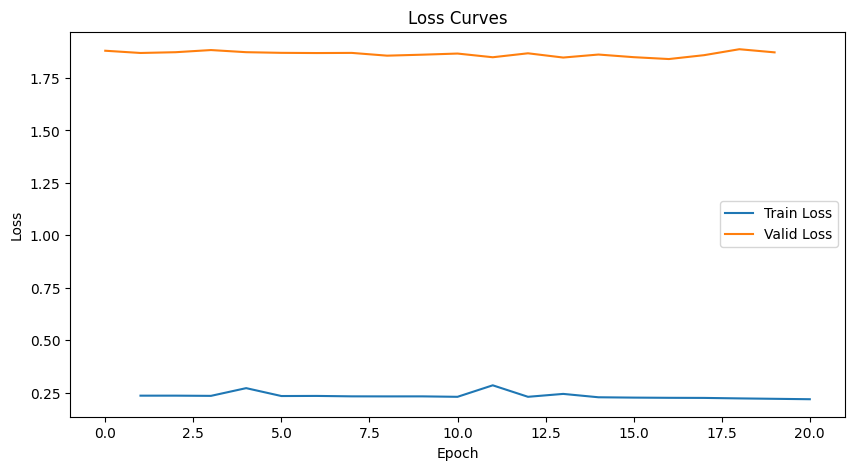
\includegraphics[width=\columnwidth]{figures/training plot.png}
    \caption{Training and validation loss plot.}
    \label{fig:plot}
\end{figure}

\begin{table}[htbp]
\centering
\caption{NCDE model performance on test set.}
\label{tab:hyperparameters}
\begin{tabular}{| l | l | l | l |}
\hline
\textbf{Method} & \textbf{MSE} & \textbf{Cross-Entropy}& \textbf{Accuracy} \\
\hline
NCDE model (final epoch) & 0.0992 & 1.7809 & 30.55 \\
\hline
NCDE model (best classify loss) & 0.0992 & 1.7809 & 30.55 \\
\hline
NCDE model (best MSE loss) & 0.0999 & 1.7913 & 0.2222 \\
\hline
\label{tab:result}
\end{tabular}
\end{table}

Further comparison between regular cubic spline and NCDE is required to determine if the model is underfitting or if the input sequences does not have enough discriminatory information.

\section{Results}

\section{Discussion}

\section*{Acknowledgments}

%% The file named.bst is a bibliography style file for BibTeX 0.99c
\bibliographystyle{named}
\bibliography{ijcai26}

\end{document}

